\documentclass[pdftex,a4paper,12pt]{report}

\usepackage[utf8]{inputenc}  % Accenten gebruiken in tekst (vb. é ipv \'e)
\usepackage{amsfonts}        % AMS math packages: extra wiskundige
\usepackage{amsmath}         %   symbolen (o.a. getallen-
\usepackage{amssymb}         %   verzamelingen N, R, Z, Q, etc.)
\usepackage[dutch]{babel}    % Taalinstellingen: woordsplitsingen,
                             %  commando's voor speciale karakters
                             %  ("dutch" voor NL)
\usepackage{eurosym}         % Euro-symbool €
\usepackage{geometry}
\usepackage{graphicx}        % Invoegen van tekeningen
\usepackage[pdftex,bookmarks=true]{hyperref}
                             % PDF krijgt klikbare links & verwijzingen,
                             %  inhoudstafel
\usepackage{listings}        % Broncode mooi opmaken
\usepackage{multirow}        % Tekst over verschillende cellen in tabellen
\usepackage{rotating}        % Tabellen en figuren roteren
\usepackage{natbib}          % Betere bibliografiestijlen
\usepackage{fancyhdr}        % Pagina-opmaak met hoofd- en voettekst

\usepackage[T1]{fontenc}     % Ivm lettertypes
\usepackage{lmodern}
\usepackage{textcomp}

\usepackage[parfill]{parskip}
\usepackage{fancyhdr}

\usepackage{lipsum}          % Voor vultekst (lorem ipsum)

% \usepackage[parfill]{parskip}
% \usepackage{fancyhdr}

%%---------- Layout ------------------------------------------------------

% hoofdingen, enz.
\pagestyle{fancy}
% enkel hoofdstuktitel in hoofding, geen sectietitel (vermijd overlap)
\renewcommand{\sectionmark}[1]{}

% lijn, wordt gebruikt in titelpagina
\newcommand{\HRule}{\rule{\linewidth}{0.5mm}}

% Leeg blad
\newcommand{\emptypage}{
\newpage
\thispagestyle{empty}
\mbox{}
\newpage
}

% Gebruik een schreefloos lettertype ipv het "oubollig" uitziende
% Computer Modern
\renewcommand{\familydefault}{\sfdefault}

% Commando voor invoegen Java-broncodebestanden (dank aan Niels Corneille)
% Gebruik: \codefragment{source/MijnKlasse.java}{Uitleg bij de code}
\newcommand{\codefragment}[2]{ \lstset{%
  language=java,
  breaklines=true,
  float=th,
  caption={#2},
  basicstyle=\scriptsize,
  frame=single,
  extendedchars=\true
}
\lstinputlisting{#1}}

%%---------- Documenteigenschappen ---------------------------------------
%% Vul dit aan met je eigen info:

% Je eigen naam
\newcommand{\student}{Nathan Baele}

% De naam van je lector, begeleider, promotor
\newcommand{\promotor}{Bert Van Vreckem}

% De naam van je co-promotor
\newcommand{\copromotor}{Selami Top}

% Indien je bachelorproef in opdracht van een bedrijf of organisatie
% geschreven is, geef je hier de naam.
\newcommand{\instelling}{---}

% De titel van het rapport/bachelorproef
\newcommand{\titel}{Beveiliging van een Windows Server 2012 R2 webserver met ASP.NET applicatie}

% Datum van indienen
\newcommand{\datum}{29 mei 2015}

% Faculteit
\newcommand{\faculteit}{Faculteit Bedrijf en Organisatie}

% Soort rapport
\newcommand{\rapporttype}{Scriptie voorgedragen tot het bekomen van de graad van\\Bachelor in de toegepaste informatica}

% Academiejaar
\newcommand{\academiejaar}{2014-2015}

% Examenperiode
%  - 1e semester = 1e examenperiode
%  - 2e semester = 2e examenperiode
%  - tweede zit = 3e examenperiode
\newcommand{\examenperiode}{Tweede examenperiode}

%%========================================================================
%% Inhoud document
%%========================================================================

\begin{document}

%%---------- Front matter ------------------------------------------------
%% Het voorblad - Hier moet je in principe niets wijzigen.

\begin{titlepage}
  \newgeometry{top=2cm,bottom=1.5cm,left=1.5cm,right=1.5cm}
  \begin{center}

    \begingroup
    \rmfamily
    
\includegraphics[width=2.5cm]{img/HG-beeldmerk-woordmerk}\\[.5cm]
    \faculteit\\[3cm]
    \titel
    \vfill
    \student\\[3.5cm]
    \rapporttype\\[2cm]
    Promotor:\\
    \promotor\\
    Co-promotor:\\
    \copromotor\\[2.5cm]
    Instelling: \instelling\\[.5cm]
    Academiejaar: \academiejaar\\[.5cm]
    \examenperiode
    \endgroup

  \end{center}
  \restoregeometry
\end{titlepage}

% Schutblad

\emptypage


\begin{titlepage}
  \newgeometry{top=5.35cm,bottom=1.5cm,left=1.5cm,right=1.5cm}
  \begin{center}

    \begingroup
    \rmfamily
    \faculteit\\[3cm]
    \titel
    \vfill
    \student\\[3.5cm]
    \rapporttype\\[2cm]
    Promotor:\\
    \promotor\\
    Co-promotor:\\
    \copromotor\\[2.5cm]
    Instelling: \instelling\\[.5cm]
    Academiejaar: \academiejaar\\[.5cm]
    \examenperiode
    \endgroup

  \end{center}
  \restoregeometry
\end{titlepage}


\begin{abstract}
% TODO: De "abstract" of samenvatting is een kernachtige (max 1 blz. voor een
% thesis) synthese van het document. In ons geval beschrijf je kort de
% probleemstelling en de context, de onderzoeksvragen, de aanpak en de
% resultaten.
Vandaag de dag hoor je regelmatig eens in het nieuws dat er een bedrijf is opgelicht door professionele hackers, oplichters die zijn binnen gedrongen in hun netwerk en gevoelige informatie hebben gebruikt om zaken te verkrijgen. Dit probleem groeit even snel als de groei van netwerken in het bedrijfsleven. Daarom is het belangrijk om een zeer goed beveiligd netwerk te hebben tegen bedreigingen van zowel binnen als buiten het bedrijf. \newline \newline

Mijn grootste doelstelling is om een overzicht te voorzien van welke soorten maatregelen er zeker moeten getroffen worden om een netwerk optimaal te beveiligen. Dit gaande van de router tot de switch tot de server. Ik wil zelf ook zo een beveiligd netwerk/server kunnen opzetten en zelf kunnen testen dat er geen enkele vorm van bekende bedreigingen binnen kan. Tot slot wil ik te weten komen of er in het bedrijfsleven wel nood en budget is voor zulke hevige beveiligingen. \newline \newline

Om dit probleem te onderzoeken heb ik op voorhand enkele onderzoeksvragen vastgesteld. Wat zijn de bekendste soorten van externe en interne bedreigingen en hoe worden deze het efficiëntst opgelost? Hoe word je router en switch zo optimaal mogelijk beveiligd? Hoe wordt de server zo goed mogelijk beveiligd? Wat zijn de voor -en nadelen van bepaalde beveiligingstechnieken? \newline 


\textbf{Zijn de 'best practices' voldoende als beveiliging tegen een externe of interne aanval? Wat is de beste manier om als administrator sporen terug te vinden van een aanval?
} (KAN NOG VERANDEREN)
\end{abstract}

\chapter*{Voorwoord}
\label{ch:voorwoord}
Deze scriptie zou niet to stand gekomen zijn zonder de hulp van mijn stagementor en co-promotor Selami Top. Ik mocht gebruik maken van zijn huidig netwerk en ik mocht enkele zaken uitproberen op zijn nieuw netwerk. Hierdoor kon ik de zaken die ik onderzocht en opgezocht had uit proberen in een echte omgeving en kreeg ik een betere kijk op een realistische beveiliging. Verder wil ik ook mijn promotor Bert Van Vreckem bedanken die mij heeft geholpen om deze bachelorproef tot stand te brengen. Zijn tips en technische kennis waren een enorme hulp om dit resultaat te bekomen. (NOG WAT TOEVOEGEN). Tot slot wil ik alle auteurs bedanken van de lectuur die ik heb gebruikt om deze scriptie te maken (LIJST VAN ALLE AUTEURS?)
% TODO: Vergeet ook niet te bedankten wie je geholpen/gesteund/... heeft

\tableofcontents

% Als je een lijst van afkortingen of termen wil toevoegen, dan hoort die
% hier thuis. Gebruik bijvoorbeeld de ``glossaries'' package.

%%---------- Kern --------------------------------------------------------

\chapter{Inleiding}
\label{ch:inleiding}

De inleiding moet de lezer alle nodige informatie verschaffen om het onderwerp te begrijpen zonder nog externe werken te moeten raadplegen \citep{Pollefliet2011}. Dit is een doorlopende tekst die gebaseerd is op al wat je over het onderwerp gelezen hebt (literatuuronderzoek). \newline \newline

Je verwijst bij elke bewering die je doet, vakterm die je introduceert, enz. naar je bronnen. In \LaTeX{} kan dat met het commando \texttt{$\backslash${cite\{\}}} of \texttt{$\backslash${citep\{\}}}. Als argument van het commando geef je de ``sleutel'' van een ``record'' in een bibliografische databank in het Bib\TeX{}-formaat (een tekstbestand). Als je expliciet naar de auteur verwijst in de zin, gebruik je \texttt{$\backslash${}cite\{\}}.
Soms wil je de auteur niet expliciet vernoemen, dan gebruik je \texttt{$\backslash${}citep\{\}}. Hieronder een voorbeeld van elk.

\cite{Knuth1998} schreef een van de standaardwerken over sorteer- en zoekalgoritmen. Experten zijn het erover eens dat cloud computing een interessante opportuniteit vormen, zowel voor gebruikers als voor dienstverleners op vlak van informatietechnologie~\citep{Creeger2009}.

\section{Probleemstelling en Onderzoeksvragen}
\label{sec:onderzoeksvragen}

% TODO: Wees zo concreet mogelijk bij het formuleren van je
% onderzoeksvra(a)g(en). Een onderzoeksvraag is trouwens iets waar nog
% niemand op dit moment een antwoord heeft (voor zover je kan nagaan).
\subsection{Zijn de "`best practices"' voldoende als beveiliging tegen een externe of interne aanval?}

Er circuleren talrijke zogenaamde "`best practices"' om een webserver te beveiligen tegen interne en externe bedreigingen. Deze "`best practices worden geïmplementeerd op een webserver en daarna wordt deze aangevallen door enkele veelgebruikte en bekende interne en externe aanvallen om te testen of deze best practices voldoende zijn.

\subsection{Wat is de beste manier om als administrator sporen terug te vinden van een aanval?}

Het spreekt voor zich dat, wanneer er zich een aanval voordoet of heeft voorgedaan, dat een netwerkbeheerder dit direct of toch zo snel mogelijk wilt te weten komen. Als er een aanval gaande is dan is het belangrijk dat de beheerder dit snel weet en dat deze snel de oorzaak vindt en weet wat er precies aan het gebeuren is. Hetzelfde geldt voor wanneer er een aanval heeft plaatsgevonden in de geschiedenis. Het is de taak van de administrator om ervoor te zorgen dat aanvallen makkelijk terug te vinden zijn ofwel manueel ofwel automatisch zodat deze tijdig kunnen onderbroken worden of niet meer zullen voorvallen.

\chapter{Methodologie}
\label{ch:methodologie}

% TODO: Hoe ben je te werk gegaan? Verdeel je onderzoek in grote fasen, en
% licht in elke fase toe welke stappen je gevolgd hebt. Verantwoord waarom je
% op deze manier te werk gegaan bent. Je moet kunnen aantonen dat je de best
% mogelijke manier toegepast hebt om een antwoord te vinden op de
% onderzoeksvraag.

Dit onderzoek bestaat uit de volgende methodiek:
\begin{enumerate}
	\item Een dergelijke basiskennis is vereist dus het verrichten van onderzoek en lezen van lectuur is een essentiële eerste stap.
	\item Opzetten van een goede testomgeving met één Windows Server 2012 R2 webserver met ASP.net-applicatie draaiende als slachtoffer, één Kali Linux-machine als aanvaller en één Windows 8.1-machine die als client fungeert. De twee Windows-machines moeten geconfigureerd worden volgens best practice-beveilging.
	\item Met behulp van penetration testing tools beveiligingsproblemen zoeken en uitbuiten. Hier wordt er vanuit gegaan dat er geen fysieke toegang is tot de server dus het betreft een externe aanval. Er wordt een lijst gemaakt met welke aanvallen er gaan gedaan worden en welke succesvol worden uitgevoerd en welke falen. Indien een aanvaal succesvol wordt uitgevoerd, dan zullen de best practices moeten aangevuld worden.
	\item Het uitvoeren van een post-mortem om sporen van inbraak bloot te leggen en kijken waar het probleem zich bevindt.
\end{enumerate}

\section{Opzetten testomgeving}
\subsection{Situering}
\begin{center}
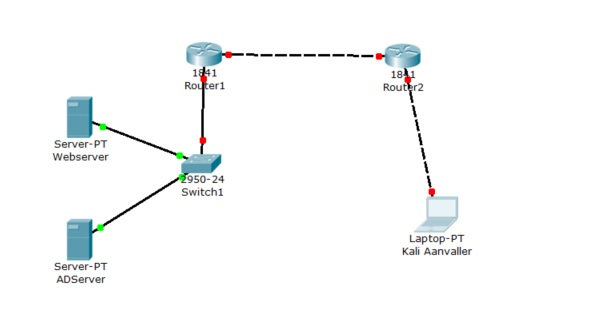
\includegraphics{img/Situatie}
\end{center}

In de afbeelding is te zien welke machines allemaal nodig zijn om dit onderzoek tot een goed einde te brengen. Ten eerste is er een Active Directory-server nodig die ook domeincontroller is in het domein en deze server is ook nog DNS-server ook. Dan is er de webserver die lid is van hetzelfde domein als de ADServer natuurlijk. Deze zijn aangesloten aan een switch en een router. Ten slotte is er ook nog een aanvallersmachine om te proberen de server te hacken. Deze is ook aangesloten aan een router op een andere locatie. Tot slot wordt er gebruik gemaakt van VMWare Workstation om al deze virtuele machines te maken met elkaar te verbinden.

\subsection{Installatie + configuratie ADServer}
De Windows Server 2012 R2-virtuele machine genaamd "`ADServer"' is de eerste die moet worden opgezet. In VMWAre Workstation wordt er 60GB geheugen gealloceerd voor deze virtuele machine samen met twee netwerkadapters en 2GB aan RAM-geheugen. Nadat Windows Server 2012 R2 is geïnstalleerd op deze virtuele machine, krijgt deze de naam "`ADServer"' en wordt deze heropgestart. Daarna kan er begonnen worden met het installeren van de nodige rollen. De eerste rol die wordt geïnstalleerd is de rol textit{Active Directory Domain Services}. Daarna wordt de ADServer opgewaardeerd naar domeincontroller in het fictieve domein "`Baele.be"'. \newline 

Op de server zijn twee netwerkadapters aanwezig, één die is verbonden met het internet (Internetadapter) en een andere die is verbonden met het LAN (LANadapter). De internetadapter staat geconfigureerd als NAT en de IP -en DNS-informatie worden alletwee automatisch aangewezen. Bij de LANadapter zijn de instellingen anders, hier staat deze configureerd als "`Custom: specific virtual network"' en wordt er gekozen om het virtuele network de naam \textit{VMnet0} mee te geven. Hierdoor moeten de IP -en DNS-instellingen handmatig geconfigureerd worden. De server krijgt al IP-adres 192.168.1.2 mee, als subnetmask 255.255.255.0, als default gateway 192.168.1.2 en als DNS-server 127.0.0.1. \newline

Het volgende dat moet gebeuren is het installeren en configureren van de DNS-rol. Dit is vrij simpel en neemt niet veel tijd in beslag. In het scherm "`DNS-beheer"' wordt er in het tabblad "`Zones voor reverse lookup"' een zone aangemaakt met de naam "`1.168.192.in-addr.arpa"' en daarna wordt er een PTR-record aangemaakt die verwijst naar de net geconfigureerde LANadapter met het juiste IP-adres. Hierna wordt de DHCP-rol geïnstalleerd en wordt er een nieuwe scope aangemaakt met de naam "`TestScope"'. Het eerste IP-adres in het bereik is 192.168.1.1 en het laatste 192.168.1.254. De adressen van 192.168.1.1 tot 192.168.1.20 worden uitgesloten voor distributie. De router is de server zelf dus het IP-adres is 192.168.1.2 net als de DNS-server. Tot slot wordt de scope geactiveerd. \newline

\subsection{Installatie + configuratie WebServer}
De installatie start op dezelfde manier als de voorgaande machine, maar in dit geval wordt de machine "`WebServer"' genoemd.

\subsection{Installatie + configuratie aanvallersmachine}
De derde en laatste virtuele machine die nodig is in dit onderzoek is de Kali Linux-aanvallersmachine. Deze is vrij makkelijk te installeren en heeft ook niet zo hoge systeemvereisten. Voor deze machine is er maar 20Gb aan gealloceerd geheugen nodig samen met 1 netwerkadapter en 512MB aan RAM-geheugen. Bij het starten van de installatie is het gemakkelijk dat er gekozen wordt voor "`graphical install"'. De meeste stappen zijn voor de hand liggend, maar bij partition disks wordt er 'guided-use entire disk' het best geselecteerd. Voor de rest zijn de overige stappen niet zo belangrijk en is de installatie zo afgerond.

%% TODO: de structuur en titel van deze hoofdstukken hangen af van je
% eigen onderzoek. Elke fase in je onderzoek kan een eigen hoofdstuk krijgen. Kies telkens een gepaste titel. ``Corpus'' is *GEEN* gepaste titel
\chapter{Opzetten server met best practises beveiliging}
´%Hier ga ik schrijven over wat de best practises zijn om een webserver te beveiligen en ga ik zeggen hoe je deze moet configureren/implementeren

\section{Inloggen}
Eén van de eerste zaken dat moet gebeuren is het uitschakelen van de inlognaam "Administrator" en een eigen administrator login maken en deze dan toevoegen aan de groep "`Administrators"' zodat deze dezelfde rechten heeft als het net uitgeschakelde account. De reden voor deze maatregel is om brute force aanvallen tegen te gaan. Elke IT'er kent het "`Administrator-account"' en deze is dan kwetsbaar voor aanvallen die proberen om het wachtwoord te kraken. Als het account is uitgeschakeld dan moet er al een accountnaam geweten zijn voordat er brute force aanvallen kunnen plaatsvinden. In dit geval is er een account aangemaakt genaamd "`BaeleAdministrator"' en is deze lid geworden van de groepen \textit{Administrators, Domeinadministrators en domeincontrollers}. Ook is het gebruikelijk dat er een complex wachtwoord wordt gebruik voor dit account. Er wordt aangeraden om hoofdletters, kleine letters, cijfers en speciale tekens te gebruiken in het wachtwoord. Een andere best practice is om het wachtwoord regelmatig, maandelijks of half jaarlijks, eens te wijzigen. Ten slotte is het ook een best practice dat er bij de groepsbeleidsobjecten wordt ingesteld dat een account wordt geblokkeerd nadat er 3x verkeerd is ingelogged. 

\section{Updates}
Nog een belangrijke onderdeel van een server met best practice beveiliging, is het constant downloaden en installeren van updates. Het is dan ook aanbevolen dat je de updates automatisch laat uitvoeren. Dit zorgt ervoor dat de server continu is voorzien van de beste beveiliging en dat alle bugs die er op die moment aanwezig zijn, zijn verdwenen. 

\section{Backup}
Het maken van geautomatiseerde backups is essentieel voor een server binnen een netwerk. Een fout, probleem of aanval kan elke moment van de dag gebeuren en als dit gebeurd moet het mogelijk zijn om het systeem terug te zetten van een eerder gemaakte backup. In de Windows Server Backup-wizard kan dit worden ingesteld voor elke ahrde schijf. In dit geval wordt er enkel elke nacht om 03:00u een backup genomen van de C-schijf. 

\section{Firewall}
Default is de firewall al vrij goed beveiligd tegen de meeste zaken. Er is echter één aanpassing die in de praktijk veel wordt toegepast en die ook door velen wordt genoemd als een best practise-instelling voor een Firewall-configuratie. Dit betreft het blokkeren van alle uitgaande verbindingen die niet overeenkomen met één van de gedefinieerde regels. Dit doe je door naar de eigenschappen te gaan en daar in alledrie de profielen de uitgaande verbindingen op "`blokkeren"' te zetten. Standaard staat dit geconfigureerd als "`toestaan"'. Voor de rest zijn er geen algemene best practices te vinden voor de Firewall.

\section{IIS}
\subsection{Modules}
In totaal bevat IIS meer dan 30 modules en deze moeten niet allemaal actief zijn. In de IIS manager kan er in het modulescherm van de geselecteerde website bepaalde modules op inactief gezet worden. In de lijst moet er beslist worden welke modules nodig zijn en de welke overbodig zijn. De overbodige modules kunnen dan worden uitgeschakeld door deze uit de lijst te verwijderen. 

\subsection{Opties methode uitschakelen}
De opties methode geeft een lijst van methodes weer die worden ondersteund door de webserver. Dit kan waardevolle informatie opleveren voor een hacker. Het is dan ook een best practice om deze methode uit te schakelen en dit gebeurd door het woord "`OPTIONS"' uit te sluiten van de \textit{HTTP Verb request filtering rules} in IIS. Dit wordt gedaan door de website te selecteren in de IIS-manager en dan dubbel te klikken op "`aanvraagfiltering"' en naar het tabblad "`HTTP-termen"' te gaan. Hier wordt als actie gekozen "`Term weigeren..."' en wordt "`OPTIONS"' ingevuld en op "`OK"' gedrukt. Nu staat deze regel als enigste in de lijst en is deze best practice in orde gebracht.

\subsection{Dynamische IP restricties}
Het inschakelen van dynamic IP restrictions module zorgt ervoor dat IP-adressen die een bepaald aantal requests hebben verzonden worden geblokkeerd. Hierdoor worden \textit{Denial of Service-aanvallen} voorkomen. Deze module inspecteert het IP-adres van elke request en zal deze requests filteren om de Ip-adressen met slechte bedoelingen tijdelijk te blokkeren. Dit kan gedaan worden door naar de IIS-manager te gaan en de naam van de website te selecteren en te dubbelklikken op "`beperkingen voor IP-adressen en domeinen"'. In het actie paneel wordt er geklikt op "`instellingen voor dynamische beperking bewerken.."' en kunnen er restricties ingevoerd worden. De eerste twee vakjes van de drie moeten worden aangevinkt en de waarden kunnen naar keuze ingevuld worden, in dit geval is "`5-20-200"' ingevuld. 

\subsection{Request Filtering Rules}
Het is altijd een goed idee om de verschillende types van HTTP-request die worden verwerkt door IIS te beperken. Door het instellen van uitsluitingen en regels kunnen potentieel gevaarlijke request er nooit doorkomen. Dit gebeurd in de IIS Manager waar de juiste website wordt gekozen en waarna er dubbel wordt geklikt op "`Requestfilters"'. Hier wordt er gegaan naar het tabblad "`regels"' en kunnen verschillende filterregels toegevoegd worden.

\subsection{Inschakkelen logs}
Door het in te schakelen van het IIS logsysteem worden verschillende HTTP-request gelogged. Indien er problemen voordoen dan kan er hier gekeken worden om een betere kennis te vergaren over het probleem. Dit kan vrij snel en simpel ingeschakeld worden door te gaan naar de IIS manager en daar de gewenste website te slecteren en op logging te klikken. Best wordt er gekozen om een nieuw bestand aan te maken want deze bestanden groeien vrij snel.

\chapter{Risico-analyse}
definitie van een risico-analyse en waarom deze nodig is en hoe deze wordt uitgevoerd.

\section{Netwerkscanner}
\cite{Jackson2010} schreef dat nmap de netwerk -en scanningtool is die de meeste beveiligingsexperts gebruiken. Deze is gratis, open source applicatie is beschikbaar op alle Windows besturingssystemen. In deze situatie wordt er ook gebruik gemaakt van deze bekende tool. Nmap kan gebruikt worden om een netwerk van alle grotes te scannen. Deze tool werkt vrij simpel, als je nmap voorziet van een IP-adres dan kan je alle "`open deuren"' of poorten te zien krijgen van een specifiek IP-apparaat of een range van IP-apparaten. Dit gebeurt door een ping sweep die de hosts zal identificeren die acief zijn op een netwerk en voor deze actieve hosts zal er gekeken worden welke services er antwoorden. \citep{Messer2007}. \newline

Met behulp van een netwerkscanner, in dit geval nmap, kan er gekeken worden welke poorten kunnen geëxploit worden. Hackers gebruiken dit om te zoeken naar open poorten waardoor ze binnen een computer of netwerk kunnen breken m.b.v. een exploit. Op de webserver zullen er meer poorten open zijn dan op de ADServer die ook domeincontroller is. Bijvoorbeeld poorten 80 en 443 zijn specifiek voor een webserver. In het geval dat er poorten open zijn die niet open moeten staan, dan kunnen deze worden gesloten door naar het takenbeheer te gaan en te kijken welke service er bij deze poort hoort. Hoort deze service niet thuis op het netwerk of op de computer, dan kan deze verwijderd worden. Dankzij het uitvoeren van een port scan kan er gekeken worden of er op een server poorten open staan die vatbaar zijn voor een aanval. Indien deze tijdig worden gevonden kan een potentiële aanval afgewend zijn.

\section{Kwestbaarheidscanner}
Nessus is volgens \cite{Jackson2010} een populaire kwetsbaarheidscanner die zoekt naar zwakke plekken in besturingssystemen, netwerkapparaten en applicaties. Deze scans gebeuren via een database zodat alle nieuwste bedreigingen direct kunnen gevonden worden. Daarom is het ook belangrijk dat Nessus wekelijks of dagelijks wordt geupdate zodat elke scan zo efficiënt mogelijk kan gebeuren. Deze soort scan is een uitgebreidere versie van de nmap-scan. \newline

Allereerst moeten er policies ingesteld worden die zullen gebruikt worden om het netwerk in te schatten. In deze sectie worden ook plugins ingesteld die het hart van Nessus voorstellen. Er kunnen duizenden plugins worden ingesteld, maar om de snelheid van de scan te verbeteren is het gebruikelijk om enkel de plugins te pakken die van toepassing zijn om het te onderzoeken netwerk. Nadat deze zijn ingesteld kan er één of meerdere IP-adressen ingegeven worden om de bijhorende apparaten te scannen. Voor elke host die is gescannend komt er een lijst met alle zwaktes op een overzichtsscherm. Deze zwaktes worden gecatalogiseerd naargelang de grootte. (Afbeelding 4-1)

\begin{figure}[h!]
\begin{center}
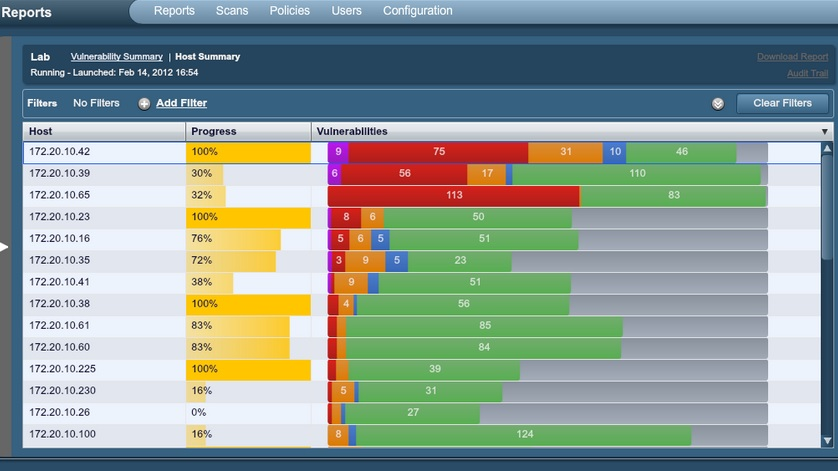
\includegraphics[scale=0.60]{img/Nessus1}
\end{center}
\caption{Voorbeeld Nessus-scan}
\end{figure}

Bij het klikken op een specifieke bedreiging is er een gedetailleerde uitleg zichtbaar. Deze uitleg bevat o.a. een voorgestelde oplossing op het probleem en hyperlinks die verwijzen naar technische documenten die het probleem toelichten. Dit is enkel een simpel gebruik van de Nessus-tool, deze kan nog veel uitgebreider gebruikt worden, maar dit is in dit geval niet aan de orde. \citep{Jackson2010}

 


\chapter{Penetration Testing}
%Hier ga ik verschillende aanvallen doen op deze server, zowel intern als extern, en ga ik mijn bevindingen noteren. Als de aanval slaagt, dan ga ik er een oplossing voor zoeken en 
%de oplossing testen, als de aanval niet slaagt, dan zijn de best practises voldoende.
\section{Applicatie laag}
\subsection{Brute force Hydra-aanval}
\subsubsection{Uitvoering en schade}
Hydra is één van de bekendste en meest gebruikte tools die Kali Linux te bieden heeft en deze is makkelijk terug te vinden op de aanvallersmachine aangezien deze tool bij de top 10 van meest gebruikte tools staat. Met Hydra kan een persoon wachtwoorden kraken van desktops of servers. Het principe is vrij simpel, de enige benodigheden zijn een Kali-machine, het ip-adres van het slachtoffer en een woordlijst die zelf kan gemaakt worden of die van het internet kan gehaald worden. In deze aanval wordt de naam van een administrator-account meegegeven en een lijst van verschillende woorden of wachtwoorden die één voor één worden uitgeprobeerd. Om deze lijst nog efficiënter te maken, kan een hacker gebruik maken van social engineering waar hij persoonlijk informatie over een gebruiker opzoekt, hetgeen zeer makkelijk is via facebook, en deze informatie dan gebruikt om wachtwoorden te vormen. Dit kan variëren van geboorteplaats tot de namen van kinderen of ouders. Al deze informatie wordt in lijsten gestoken met verschillende soorten combinaties om een groter succesratio te kennen. \citep{Wilde2013} \newline 

Voordat deze aanval kan uitgevoerd worden moet de aanvaller eerst de naam van het administrator-account weten. Standaard is dit "`Administrator"' en als netwerkbeheerders dit niet aangepast hebben dan is het zeer makkelijk om met deze aanval binnen te dringen. In dit geval beschikt de aanvaller over het eigen gemaakte account met de naam "`BaeleAdministrator"'. In de aanvallersmachine wordt er allereerst een woordenlijst gedownload of aangemaakt. In dit geval wordt er een zelfgemaakte woordenlijst gebruikt aangezien zo een internetlijst 100 000'en verschillende combinaties hebben die zeer lang duren om helemaal door te lopen. In dit geval bevat de zelfgemaakte woordenlijst 5 woorden: "`test, test123, Baele123, groen, bos"'. In dit geval is Baele123 het echte wachtwoord. Daarna wordt er in het terminalvenster dit lijntje ingetyped: "`\textit{hydra -t 1 -l BaeleAdministrator -P /root/woordenlijst.txt. -vV <IP-ADRES slachtoffer> ftp}"'. Daarna wordt elk woord in de lijst apart uitgeprobeerd totdat er een juiste combinatie is of tot de lijst doorlopen is. \newline 

De schade die deze aanval aan kan richten is immens. Bij een succesvolle aanval weet de aanvaller het wachtwoord van een account met administrator rechten. Hiermee kan hij zich aanmelden via o.a. verbinding met extern bureaublad en kan de aanvaller aan alles wat zich op een server bevindt. Het spreekt voor zich dat dit niet goed is en dat dit ervoor kan zorgen dat er geheime bestanden worden gestolen of dat het netwerk wordt platgegooid en noem maar op.

\subsubsection{Bescherming en preventie}
De best practices die eerder besproken zijn, zijn voldoende om deze aanval af te weren. Hoe complexer een wachtwoord is, hoe kleiner de kans is dat het wachtwoord zich in de woordenlijst zal bevinden. Er bestaan natuurlijk gigantisch grote woordenlijsten waar bijna alle mogelijke combinaties in gebruikt worden, maar deze duren veel langer om uit te voeren. Hoe complexer het wachtwoord, hoe langer de aanval ook moet duren dus hoe meer kans er is dat de aanval wordt opgemerkt of wordt onderbroken. \newline 

Ook een best practice is om het default account "`Administrator"' uit te schakelen en een zelfgemaakt account te maken. Als dit wordt gedaan dan moet een aanvaller al kennis hebben over het netwerk en de server om te weten welk account er kan gekraakt worden. Als het default account wordt gebruikt dan kan iedereen op elke plaats in de wereld binnen breken zonder dat de persoon iets weet van een server. Dit in combinatie met een groepsbeleidobject die het account blokkeert na 3 foutieve pogingen zorgt ervoor dat deze aanval geen schijn van kans heeft.

\section{Transportlaag}
\subsection{Sockstress DDOS-aanval}
\subsubsection{Uitvoering en schade}
Een fysieke machine kan onbruikbaar gemaakt worden door een simpele aanval genaamd "`sockstress"'. Deze aanval heeft de laatste tijd enorm gewonnen aan populariteit in het hackersmilieu en dus ook in de kringen van netwerkbeveiligers. Deze methode wordt gebruikt om servers aan te vallen over het internet door middel van TCP. Deze methode zorgt ervoor dat het lokale geheugen zoveel aanvragen moet behandelen dat deze langzaam maar zeker volloopt zodat de server vastloopt en onbruikbaar wordt. Dit wordt ook wel een DOS (Denial Of Service)-aanval genoemd. \newline 

Op de aanvallersmachine, in dit geval de eerder geconfigureerde Kali Linux-machine, worden er twee verschillende "`command lines (cmd)"' geopend. In de eerste cmd wordt er \textit{"`nmap <ipadres slachtoffer>"'} getyped om te kijken welke poorten van het slachtoffer die open zijn. De open poorten worden dan ergens genoteerd want deze zijn later nog nodig. Nadat deze zijn genoteerd, wordt er een script genaamd \textit{"`./arppoi"'} geopend in dit terminalvenster. Dit scriptje is te vinden op het internet en de code is te zien in de appendix. De bedoeling van dit script is ARP spoofing. ARP spoofing is een techniek die door veel hackers wordt gebruikt en waar er vermomde ARP-berichten in een lokaal netwerk worden verzonden. De bedoeling is om het MAC-adres van de aanvaller te associëren met het IP-adres van een host, bijvoorbeeld een default gateway of server, zodat al het verkeer dat bedoelt is voor dat specifieke adres naar de aanvaller wordt verzonden. \newline 

Nu dat scriptje draait in het een terminalvenster, hoeft er in het andere venster maar één lijntje ingevuld worden. \textit{"`./sockstress -A -C -1 -d <IP van target> -m -1 -Ms -p <alle opgeschreven poorten> -r 100000 -s 172.16.246.0/25 -vv"'}. Dit werkt ook alleen maar als sockstress is gedownload en als je navigeert naar de sockstress-map. Nu kan er gekeken worden naar de server en is er te zien dat het RAM-geheugen dat in gebruik is op de server exponentieel aan het stijgen is. Als dit de maximume waarde bereikt dan zal de server vastlopen en kan er niets meer op gedaan worden. De engiste manier om de server terug aan de praat te krijgen is door manueel de uit-knop in te drukken en hem dan weer op te starten.

\subsubsection{Bescherming en preventie}
De best practices die op de server zijn geïmplementeerd zijn in dit geval niet voldoende en dus moet er een oplossing gevonden worden. De oplossing in dit geval is vrij simpel. Dit kan gedaan worden door het blokkeren van een IP-adres als het meer dan 10 connecties met een poort maakt in minder dan 30 seconden. Dit wordt gedaan door een simpel lijntje in te typen in de router command line \textit{"`iptables -I INPUT -p tcp --dport 80 -m state --state NEW -m recent --update --seconds 30 --hitcount 10 -j DROP"'}. Aangezien de server enkel handmatig kan worden afgesloten, is de kans reeël dat er gegevensverlies is. Daarvoor is het belangrijk dat dit direct wordt bekeken nadat de server opnieuw is opgestart zodat er direct een restore kan plaatsvinden als dit nodig is. Hiervoor zijn de best practices wat betreft back-ups wel voldoende. 

\section{Internetlaag}

\section{Netwerklaag}
\subsection{Malware applicaties}
\subsubsection{Uitvoering en schade}
Malware is een afkorting van "`malicious software"' en betreft alle software die als bedoeling heeft om een netwerk of computere schade toe te brengen. Er zijn verschillende soorten malware waaronder virussen en spyware behoren tot de bekendste. \citep{Moir2003}. In dit geval wordt er een simpel malware-bestand aangemaakt en op de server geplaatst. Hier wordt er gesimuleerd dat de administrator een schadelijk stukje software download op het internet en deze dan laat uitvoeren. \newline

Door het typen van de volgende tekst in een kladblokbestand kan er een virus aangemaakt worden: "`@echo off :A start virus.bat start notepad.ext goto A"' en sla dit bestand op als "`virus.bat"'. Dit simpel virus zorgt ervoor dat het RAM-geheugen van een computer of server binnen de minuut helemaal volloopt. Het programma start elke keer een commandprompt op en elke keer als dit gebeurd wordt er ook een nieuwe kladblokapplicatie geopend. Dit gebeurd oneindig veel keer tot het RAM-geheugen vol zit en de server of computer vastloopt. Hierna kan een apparaat enkel manueel worden afgesloten om het weer aan de praat te krijgen.


\textbf{LOGS}

\chapter{Post mortem}
%Hier ga ik een aanval uitvoeren en ga ik kijken waar je dit precies kan terugvinden als administrator of waar je kan het kan zien als het aan het gebeuren is.
\section{Manueel}
\subsection{RAM-geheugen}
Manueel kan er makkelijk gekeken worden naar het RAM-geheugen dat wordt gebruikt door "`ctrl+alt+del"' in te drukken of door met de rechtermuisknop te drukken op het Windows-logo linksonder op het scherm en "`Taakbeheer"' te selecteren. Hierin zijn er verschillende tabbladen en het RAM-geheugen kan gevonden worden in het tabblad "`Prestaties"' waarna er kan geklikt worden op "`Geheugen"' in de linkerkolom. In dit venster is het geheugengebruik voor de laatste 60 seconden zichtbaar en wordt deze elke seconden ververst. Als de curve per seconde omhoog gaat dan kan er sprake zijn van een Sockstress DDOS-aanval en kan er tijdig gehandeld worden. Het manueel bekijken van het RAM-geheugen kan handig zijn als de server opeens trager begint te werken om te kijken of het probleem niet hier ligt.

\section{Automatisch}
\subsection{Prestatiemeter}
Met behulp van de prestatiemeter-tool kunnen bepaalde zaken makkelijk in de gaten gehouden worden. In de prestatiemeter kunnen er gegevensverzamelaarset aangemaakt worden naar persoonlijke voorkeur die het mogelijk maken om elk aspect apart onder de loep te nemen en deze in log files op de slaan.

\subsubsection{RAM-geheugen}
De eerste gegevensverzamelaarset die zeer handig is om te maken is één die het gebruik van het RAM-geheugen in de gaten houdt. Deze kan worden ingesteld door allereerst naar de tool "`prestatiemeter"' te gaan en te rechterklikken op "`Prestatiemeter"' onder het tabblad "`controlehulpprogramma's"'. Daarna moet er onder de keuze "`Nieuw"' gekozen worden voor "`gegevensverzamelaarset"'. Nu kan er een gepaste naam gekozen worden voor deze set, in dit geval is "`RAMGeheugen"' een goede naam aangezien we hier het RAM-geheugen gaan bekijken. Bij de volgende keuzes mag er 2x op "`volgende"' gedrukt worden. \newline

Nu is de set aangemaakt en is deze terug te vinden onder het tabblad "`Gedefinieerd door de gebruiker"' en moet er hier op gedubelklikt worden tot "`Logboek voor Systeemmonitor"' zichtbaar is en dan moet er hier op gedubbelklikt worden. Nu zijn de eigenschappen van de set zichtbaar en kunnen er via "`Toevoegen"' specifieke paramters toegevoegd worden. In dit geval is het handig om naar "`Geheugen"' te gaan en daar te kiezen voor "`Beschikbare megabytes"' en "`Percentage toegewezen bytes in gebruik"'.	Nadat deze zaken zijn toegevoegd kan er 2x geklikt worden op de OK-knop. Nu moet er met de rechtermuisknop op de juist aangemaakt set geklikt worden om dan op "`starten"' te klikken, dit een 10-tal minuten te laten lopen en daarna op "`stoppen"' te drukken. Nu kan er gekeken worden naar het tabblad "`rapporten"' en "`gedefinieerd door de gebruiker"' naar wat deze actie juist heeft opgebracht. In dit scherm is er een bestand zichtbaar (met de bijhorende datum) die bij het dubbeklikken alle paramters laat zien met de bijhorende tijd in een mooie grafiek. Hier is duidelijk wanneer precies er pieken zijn in het gebruik van het RAM-geheugen en wanneer deze precies een bepaalde grens overschrijdt.

POLYMON IS EEN IDEE.


\chapter{Notities}
Hier hou ik de zaken bij die ik al heb uitgetest, maar die ik nog niet bij 1 van de 3 hoofdstukken heb geplaatst. Dit is mijn tijdelijke "dump" waar ik test zaken schrijf voor deze bij de echte hoofdstukken terecht komen.
\newpage
Post mortem kan opgedeeld worden in manueel en automatisch. Bij automatisch worden logs aangemaakt als er een regel is overschreden.


\chapter{Conclusie}
\label{ch:conclusie}

% TODO: Trek een duidelijke conclusie, in de vorm van een antwoord op de
% onderzoeksvra(a)g(en). Reflecteer kritisch over het resultaat. Zijn er
% zaken die nog niet duidelijk zijn? Heeft het ondezoek geleid tot nieuwe
% vragen die uitnodigen tot verder onderzoek?



\bibliographystyle{apa}
\bibliography{NathanBP}

%%---------- Back matter -------------------------------------------------

\listoffigures
\listoftables

\end{document}
